\subsection{Bildegjenkjenning}

Vi ble anbefalt å bruke OpenCV av Kongsberg, et open source softwarebibliotek som brukes til bearbeiding av bilder og video. I tillegg til bruken av OpenCV ble vi oppfordret til å bruke Matlab for å programmere. Noen på gruppa hadde erfaringer i Matlab fra før, så vi betraktet ikke dette som noe stort problem.

For å bruke Matlab og OpenCV sammen trengte vi et annet open source prosjekt som het ``mexopencv''. Vi forsøkte en stund å få dette til å fungere, men vi hadde problemer med å sette opp C++, OpenCV og Matlab på en slik måte at mexopencv kunne bruke alle disse ressursene. Noe som førte til ekstra problemer var at de som hadde ansvaret for å begynne med programmeringen satt på to ulike operativsystemer og dermed opplevde forskjellige feilmeldinger underveis. 

Til slutt valgte vi å gå for en løsning hvor vi ikke brukte Matlab. Dette førte til at vi raskt kunne komme igang med utviklingen av bildegjenkjenning og hadde en enkel løsning oppe i løpet av noen dager.

\subsubsection{Første steg}

Den første implementasjonen av gjenkjenningen baserte seg på å konvertere en frame av videoen fra det normale fargespekteret RGB, se figur [\ref{fig:firstiterationrgb}], til et fargespektrum som het HSV\footnote{Hue, Saturation and Value} som vist i figur [\ref{fig:firstiterationhsv}].

\begin{figure}[h!]
	\centering
	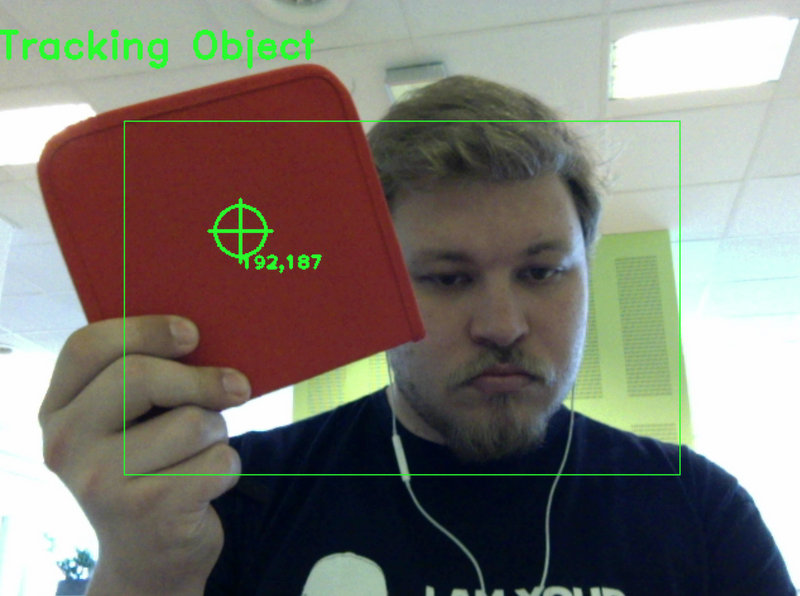
\includegraphics[scale=0.45]{img/first-rgb.jpg}
	\caption[First iteration RGB image]{Frame from video in plain RGB}
	\label{fig:firstiterationrgb}
\end{figure}

\begin{figure}[h!]
	\centering
	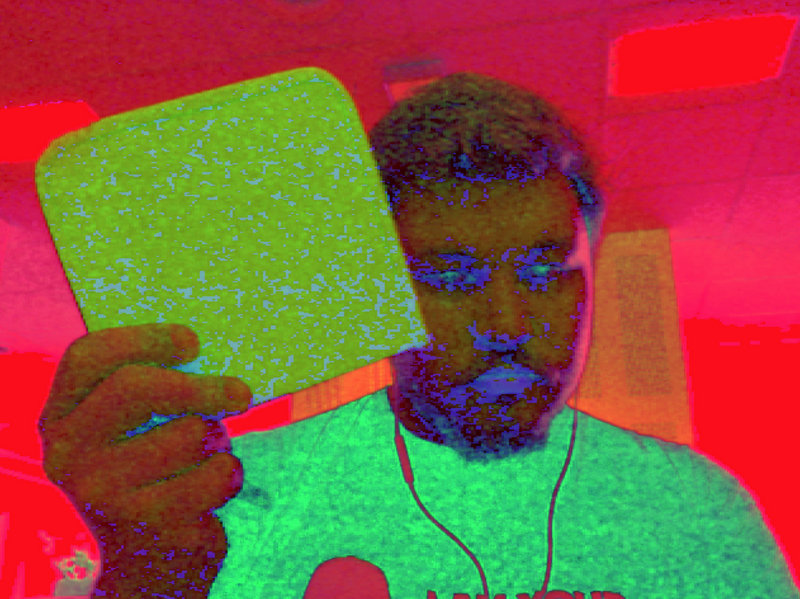
\includegraphics[scale=0.45]{img/first-hsv.jpg}
	\caption[First iteration HSV image]{Frame from video cast to HSV}
	\label{fig:firstiterationhsv}
\end{figure}

HSV baserer seg ikke på blandingen av farger, men bruker nyanser, metningsgrad og lysverdier for å vise en farge . Matrisen med fargekoder som skapes av konverteringen til HSV fører til en skarpere kontrast mellom farger, og gjør jobben med å filtrere vekk uønskede elementer lettere. Vi behandlet deretter matrisen med et filter, som vi manuelt stilte inn med maksimum- og minimumverdier for henholdsvis Hue, Saturation og Value, vist i figur [\ref{fig:sliders}]. Etter at matrisen hadde passert gjennom filteret satt vi igjen med et binært bilde, der fargene som passerte gjennom filteret er gjengitt som hvitt, mens alle andre farger er svarte slik det er vist i figur [\ref{fig:firstiterationbinary}].

\begin{figure}[h!]
	\centering
	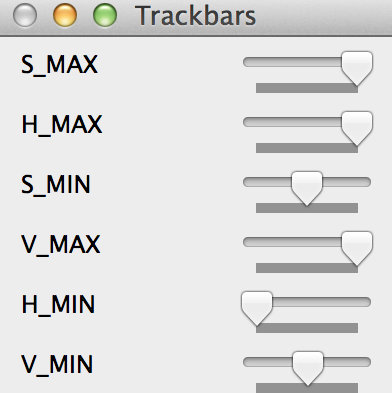
\includegraphics[scale=0.45]{img/sliders.jpg}
	\caption[Sliders to adjust HSV thresholds]{Sliders to adjust HSV thresholds}
	\label{fig:sliders}
\end{figure}

\begin{figure}[h!]
	\centering
	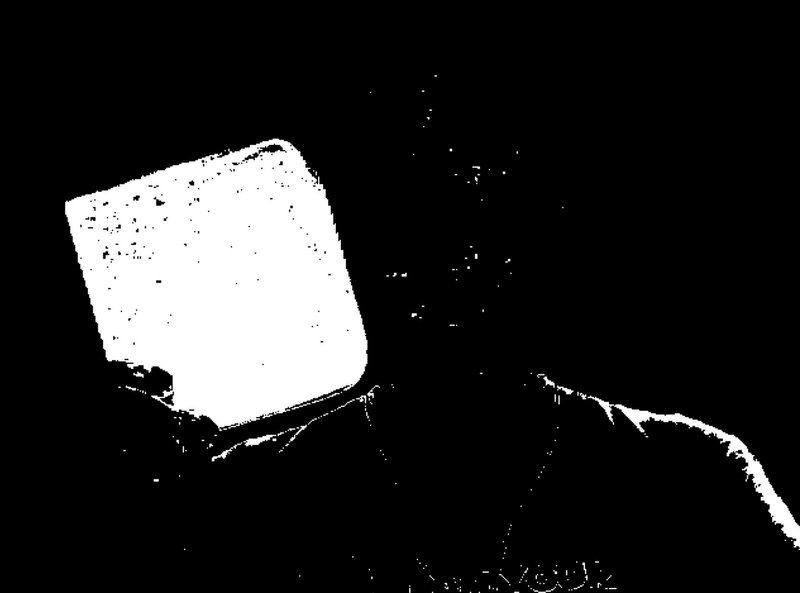
\includegraphics[scale=0.45]{img/first-binary.jpg}
	\caption[First iteration binary mage]{The resulting binary image after filtering HSV image}
	\label{fig:firstiterationbinary}
\end{figure}

\subsubsection{Andre steg}

I det første steget klarte vi å fange opp et objekt, men som man kan se i figur [\ref{fig:firstiterationbinary}] er det mye støy i bildet. Vi implementerte derfor en smoothingalgoritme som gikk over det binære bildet og fjernet mindre ansamlinger med punkter og fremhevet de som var større. Dette førte til at vi fikk et renere bilde, med færre og tydeligere objekter. Dette gjorde det betydelig lettere å fange opp de enkelte objektene i bildet og finne det største av dem.

Resultatet kan man se i figur [\ref{fig:seconditerationbinary}] 

\begin{figure}[h!]
	\centering
	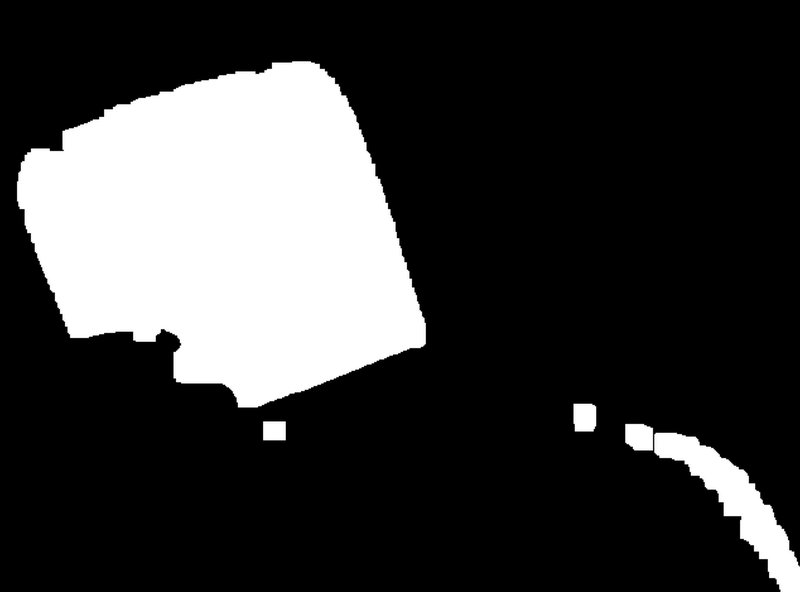
\includegraphics[scale=0.45]{img/second-binary.jpg}
	\caption[First iteration binary mage]{The resulting binary image after filtering HSV image}
	\label{fig:seconditerationbinary}
\end{figure}

\subsubsection{Tredje steg}

Etter at vi hadde jobbet en del med systemet fant vi ut at det var tungvindt å stille inn verdiene som skulle følges hver gang. Løsningen ble da at vi implementerte et enkelt kommandogrensesnitt som kunne be programmet om å følge etter fargen som befant seg i sentrum av bildet, som vist i figur [\ref{fig:commandmenu}]

\begin{figure}[h!]
	\centering
	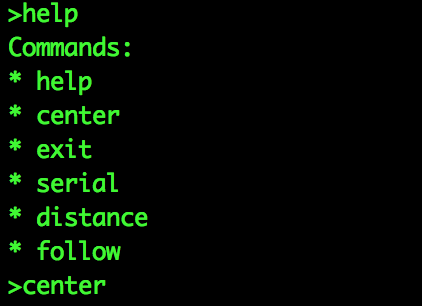
\includegraphics[scale=0.8]{img/command-menu.png}
	\caption[]{The command menu}
	\label{fig:commandmenu}
\end{figure}

\subsection{Konstruksjon av riggen}

Tekst her

\subsection{Styring av rigg + bildegjenkjenning}

Tekst her